\clearpage
\section{Domain Model}
The domain model displays the relationships between the smaller components related to feature computation.

\begin{figure}[h]
    \centering
    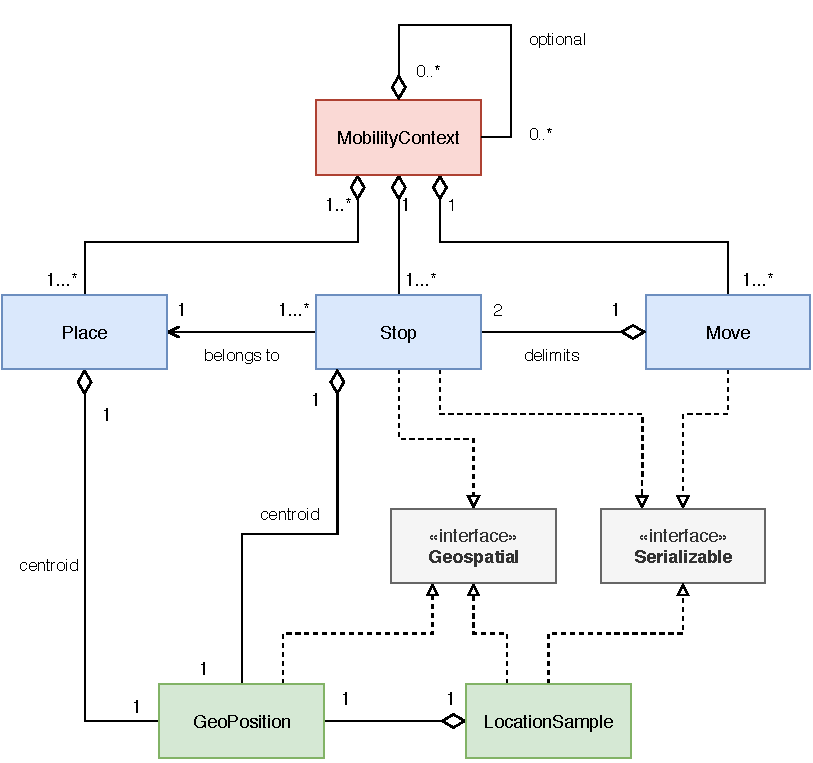
\includegraphics[width=0.7\textwidth]{images/diagrams/data-model-diagram.pdf}
    \caption{UML diagram for the classes used in the \textit{Mobility Features Package}}
    \label{fig:uml-diagram}
\end{figure}

In order to capture the data model in an object-oriented programming language, a the UML diagram shown in Figure \ref{fig:uml-diagram} was maintained as the implementation went along in order to keep track of relationships between the classes.\\

A \textbf{GeoPosition} represents a 2D position on the Earth's surface with a geographical \textit{latitude} and \textit{longitude}.\\

A \textbf{Location Sample} is a time-stamped \textit{GeoPosition}. By having a time-stamp, a collection of Location Samples may be ordered and grouped by the time of day. In essence, the class is a Data Transfer Object (DTO) as defined by Fowler \cite{fowler-PEEA} [p. 401] which is used to transfer GPS data from an arbitrary Location plugin to the \textit{Mobility Features Package}.\\

An \textbf{Hour Matrix} class is used to calculate the \textit{Routine Index} feature, as well as to identify the \textit{Home Cluster}, which is the place most visited during 00:00 and 06:00. An Hour Matrix is constructed from a list of \textit{Stops} which all have the same date.\\

\textbf{Stop} is a centroid of a data point cluster (i.e. a GeoPosition) with an arrival- and departure timestamp, and a place ID indicating which place it belongs to.\\

A \textbf{Place} is defined by a GeoPosition computed from a list of \textit{Stops} and found with the DBSCAN algorithm. Many Stops can belong to the same Place, but a Stop can only belong to one specific place.\\

A \textbf{Move} is constructed from a pair of \textit{Stops} as well as the set of \textit{Location Samples} that was sampled in the time interval between the two \textit{Stops}. This set of Location Samples is the path the user took between the two \textit{Stops}.\\

A \textbf{Mobility Context} is a the component which holds all the mobility features. This includes the location features (i.e. stops, places and moves) as well as the derived features. The component is created from daily stops and moves as well as a list of places for the whole period. In addition, a set of Mobility Contexts from previous days needs to be provided if the Routine Index feature is to be calculated, but is optional. \\

The \textbf{GeoSpatial (Interface)} forces any component implementing it to have a GeoPosition. This allows the Haversine distance to be calculated between components of different types.\\

The \textbf{Serializable (Interface)} forces any component implementing it to be serializable and deserializable. This is the case for GeoPositions, LocationSamples, Stops and Moves.
